\documentclass[a4paper]{article}
\usepackage{a4wide}
\usepackage{amsmath}
\usepackage{amsfonts}
  \DeclareMathOperator*{\argmax}{arg\,max}
  \newcommand{\ex}[1]{{\mathbb E}\left[ #1 \right]}
  \newcommand\norm[1]{\left\lVert#1\right\rVert}
\usepackage{booktabs}
\usepackage{csquotes}
\usepackage{upquote}
\usepackage{float}
\usepackage{graphicx}
\usepackage{enumerate}
\usepackage{subcaption}
\usepackage{xcolor}


\title{Pattern and Speech Recognition WS2015-16 \\ Exercise 7}
\author{Atanas Poibrenski(2554135), Marimuthu Kalimuthu(2557695), Furkat Kochkarov(2557017)}

\begin{document}

\maketitle 
\begin{center}
	\textbf{Decision Trees}
\end{center}

\section*{Exercise 1}
\begin{enumerate}
	\item[ \textbf{1} ] Done.
	\item[ \textbf{2} ] See ``data\_preparation.m"

	\begin{figure}[H]
		\begin{center}
			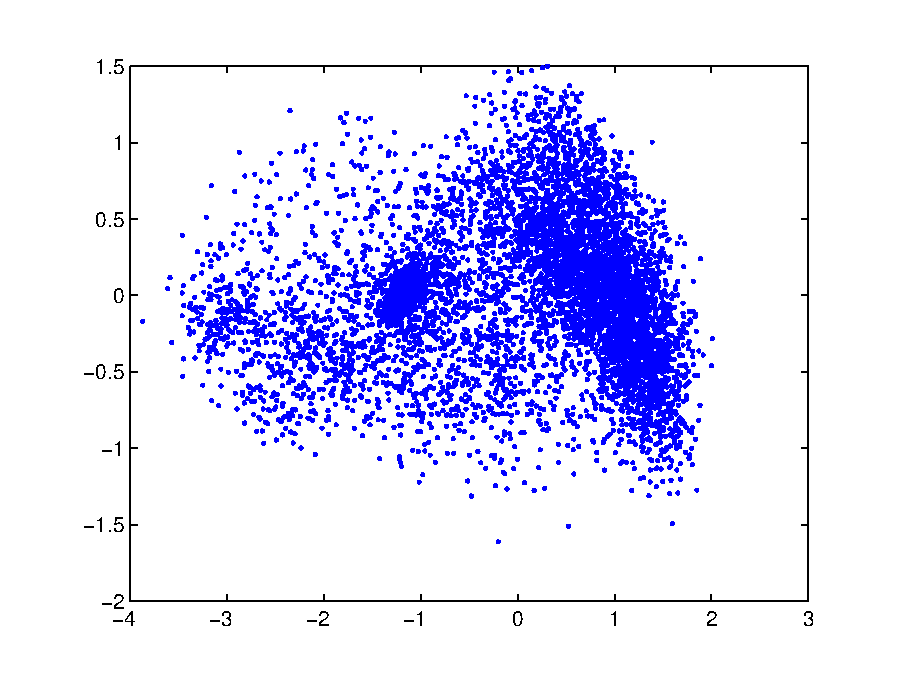
\includegraphics[width=0.9\textwidth]{data_plot.eps}
			\caption{Transformed data distribution}\label{fig:transdata}
		\end{center}
	\end{figure}

	\item[ \textbf{3} ] See ``GMM.m"
	\item[ \textbf{4} ] See ``GMM.m"
	\item[ \textbf{5} ] See ``GMM.m"
	\item[ \textbf{6} ] See ``GMM.m". We calculated the covariance matrix of the transformed data in (2) and from that we can observe that it is indeed a diagonal matrix.
	
		\begin{figure}[H]
			\begin{center}
				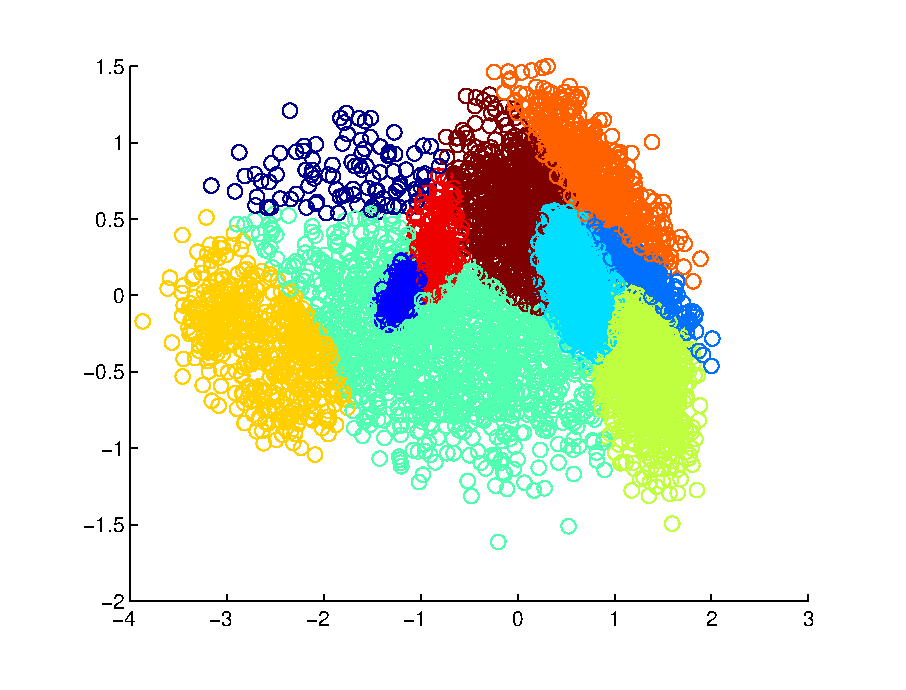
\includegraphics[width=0.8\textwidth]{GMM_K10_2.eps}
				\caption{GMM clusters(run-3) for K=10}\label{fig:gmm_k10_2}
			\end{center}
		\end{figure}

		

\end{enumerate}

\section*{Exercise-2; BONUS}
		

\end{document}
